\begin{center}
\textit{by A. Benaglia, M. Bengala, O. Bondu, L. Borgonovi, S. Braibant, L. Cadamuro, A. Carvalho, C. Delaere, M. Delcourt, N. de Filippis, E. Fontanesi, M. Gallinaro, M. Gouzevitch, J. R. Komaragiri, D. Majumder, K. Mazumdar, F. Monti, G. Ortona, L. Panwar, N. Sahoo, R. Santo, G. Strong, M. Vidal, S. Wertz}
\end{center}

The work described in this section studies the prospects for \HH production at the HL-LHC exploring five decay channels \bbbb, \bbtt, \bbWW ($\PW\PW\to\ell\nu\ell'\nu'$ with $\ell,\ell' = \Pe,\Pgm$), \bbgg, and \bbZZ ($\PZ\PZ\to\ell\ell\ell'\ell'$ with $\ell,\ell' = \Pe,\Pgm$).
The corresponding branching fractions and the total number of \HH events expected to be produced at the HL-LHC assuming $\sqrt{s} = 14\TeV$ and an integrated luminosity of $3000\fbi$ are reported in Table~\ref{sec3:CMSHH:tab:br_nevent}.

\begin{table}[h]
  \begin{center}
    \caption{Branching fraction of the five decay channels considered in the CMS \HH prospects, and corresponding number of events produced at the end of HL-LHC operations assuming $\sqrt{s} = 14\TeV$ and an integrated luminosity of $3000\fbi$. The symbol $\ell$ denotes either a muon or an electron. In the \bbWW decay channel, $\ell$ from the intermediate production of a $\tau$ lepton are also considered in the branching fraction.}
    \label{sec3:CMSHH:tab:br_nevent}
    \begin{tabular}{l  ccccc}
        \hline
        Channel            & $\bbbb$ & $\bbtt$ & $\bbWW(\ell\nu\ell\nu)$ & $\bbgg$ & $\bbZZ(\ell\ell\ell\ell)$ \\
        $\mathcal{B}$ [\%] & 33.6    & 7.3     & 1.7                    & 0.26    & 0.015\\
        Number of events   & 37000   & 8000    & 1830                   & 290     & 17\\
        \hline      
    \end{tabular}
  \end{center}
\end{table}

A parametric simulation based on the \delphes~\cite{Delphes} software is used to model the CMS detector response in the HL-LHC conditions.
The \delphes simulation accounts for the effects of multiple overlapping hadron interactions (``pileup'') by overlapping simulated minimum-bias events with on average 200 interactions per bunch crossing.
The performance of reconstruction and identification algorithms for electrons, muons, tau decays to hadrons (\tauh) and a neutrino, photons, jets (including the identification of those containing heavy flavour particles), and the missing transverse momentum vector \ptvecmiss is parametrised based on the  results obtained with a full simulation of the CMS detector and dedicated reconstruction algorithms.


\paragraph{The $\HH\to\bbbb$ channel}

While characterised by the largest branching fraction among the $\HH$ final states, the \bbbb decay channel suffers from a large contamination from the multijet background that makes it experimentally challenging.
Two complementary strategies are explored here to identify the signal contribution.
For those events where the four jets from the $\HH\to\bbbb$ decay can all be reconstructed separately, also referred to as the ``resolved'' topology, the usage of multivariate methods is explored to efficiently identify the signal contribution in the overwhelming background.
In cases where the invariant mass of the $\HH$ system, $m_{\HH}$, is large, the high Lorentz boost of both Higgs bosons may results in a so-called ``boosted'' event topology where the two jets from a $\Hbb$ decay overlap and are reconstructed as a single, large-area jet.
Resolved topologies correspond to the large majority of SM \HH events, giving the largest sensitivity on this signal.
Boosted topologies help to suppress the multijet background and provide sensitivity to BSM scenarios where the differential \HH production cross section is enhanced at high $m_{\HH}$ by the presence of $\Pg\Pg\HH$ and $\PQt\PQt\HH$ effective contact interactions.

In the resolved topology, events are pre-selected by requiring four jets with $\pt > 45~\GeV$ and $|\eta| <$ 3.5 that satisfy the medium b-tagging working point, corresponding to a b jet identification efficiency of approximately 70\% for a light  flavour and gluon jet misidentification rate of  1\%.
Triggers are assumed to be fully efficient in the phase space defined by these selection.
While this appears to be compatible with current upgrade studies of the CMS trigger system, scenarios where the minimal jet trigger \pt threshold is increased have been studied, and the loss in sensitivity corresponds to approximately 10\% and 25\% for a 10 and 30\GeV increase, respectively.

The four selected b tagged jets are combined into the two Higgs boson candidates $\PH_1$ and $\PH_2$, choosing the pairs of jets with the minimal invariant mass difference.
The invariant mass of the two Higgs candidates is required to satisfy the relation:
\begin{equation}
\sqrt{ \left( \text{m}_{\PH_1} - 120\GeV\right)^2 + \left( \text{m}_{\PH_2} - 120\GeV\right)^2 } < 40\GeV
\end{equation}
i.e. a circular selection where the center and radius are chosen based on the expected response and resolution of the CMS detector.
The center in both cases is below the Higgs boson mass because of the energy lost in B hadron decays involving neutrinos that escape detection.

Because of the very large QCD multijet background, a multivariate discriminant, in the form of a boosted decision tree (BDT), is trained to identify the \HH signal contribution and used as the discriminant variable.
Other background processes considered are \ttbar and single Higgs boson production.
The output of the BDT discriminant is shown in Fig.~\ref{sec3:CMSHH:fig:bbbb_BDT}.

\begin{figure}[!htb]
\centering 
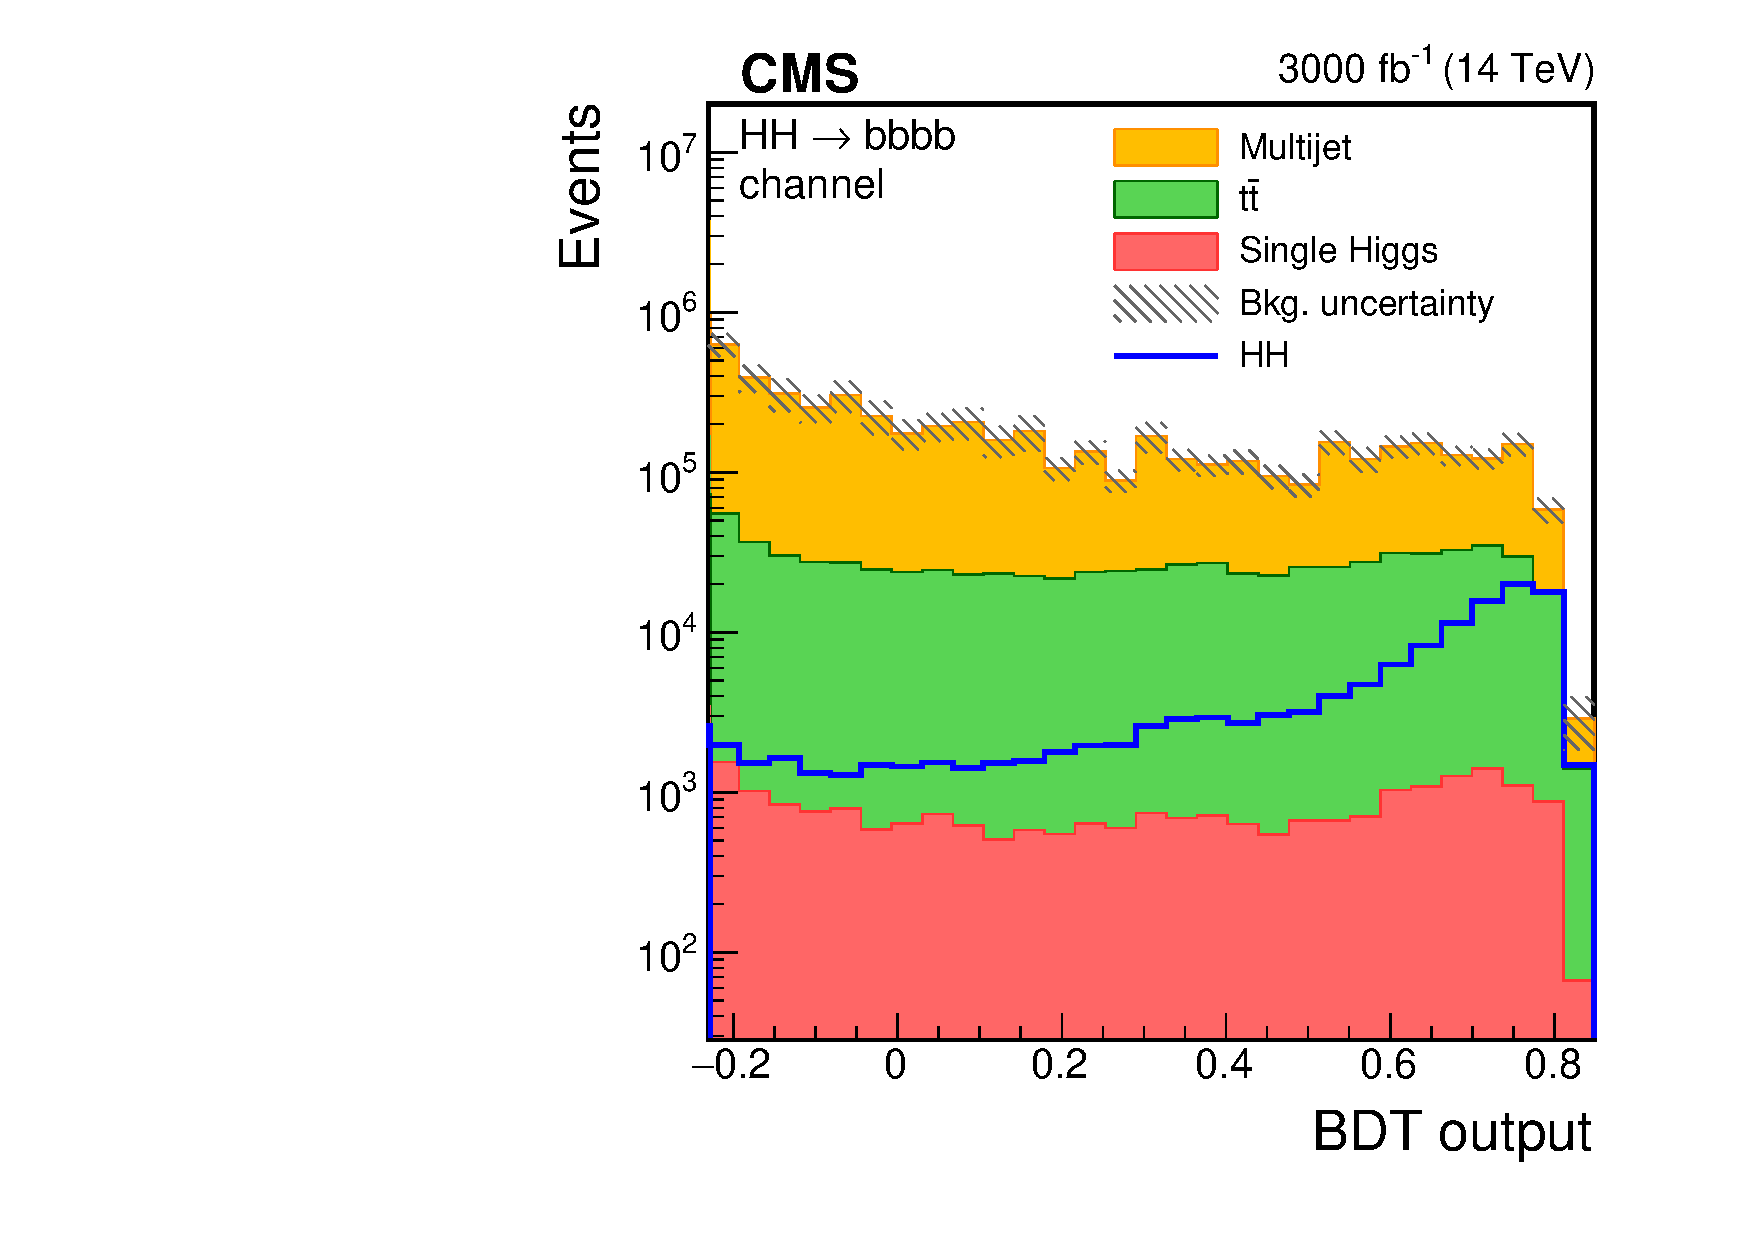
\includegraphics[width=0.5\textwidth]{\main/section3/plots/CMS/plot_BDTG_6_masscut_finalsel_log.pdf}
\caption{BDT output distribution for the signal and background processes considered in the \bbbb resolved search.} 
\label{sec3:CMSHH:fig:bbbb_BDT} 
\end{figure}

The boosted topology offers a good handle to investigate effective Higgs boson contact interactions predicted in BSM scenarios that enhance the \HH production cross section at high $m_{\HH}$ values.
For that reason, the prospects in this channels focus on anomalous couplings and make use of the shape benchmarks signals already described on section \fixme{section ref}.
Large radius jets, clustered with the anti-$k_\text{T}$ algorithm with a cone radius of 0.8 (AK8 jets), are used to identify the  overlapping b jets.
The event is required to contain at least two AK8 jets with $\pt > 300\GeV$ and $|\eta| < 3$.
The two highest \pt jets are chosen in case multiple candidates satisfy such requirements.
The soft drop~\cite{Dasgupta:2013ihk,Larkoski:2014wba} jet grooming algorithm is used to remove soft and collinear components of the jet and retain the two subjets associated with the showering and hadronization of the two b quarks from the $\PH\to\PQb\PAQb$ decay.
A selection is applied on the N-subjetiness variable~\cite{Thaler:2011gf} to reduce the background contamination, mostly represented by dijet production from QCD interactions.
Algorithms for the b jet identification are applied on the subjets with a working point corresponding to an efficiency of about 49\% for genuine b jets for a misidentification rate of light flavour and gluon jets of about 1\%.
Events are divided in two categories if they contain exactly three (3b category) or exactly four (4b category) b-tagged subjets.

The invariant mass of the two selected AK8 , $M_{JJ}$, is used to look for the presence of a signal. Its distribution is shown in Fig.~\ref{sec3:CMSHH:fig:bbbb_boosted} for the two event categories.

\begin{figure}[!htb]
\centering 
\includegraphics[width=0.5\textwidth]{\main/section3/plots/CMS/TODO.pdf}
\caption{Invariant mass of the two selected AK8 jets in the boosted \bbbb \HH serach.\fixme{placeholder} } 
\label{sec3:CMSHH:fig:bbbb_boosted} 
\end{figure}



\paragraph{The $HH \rightarrow b\bar{b}\tau\tau$ channel}

The $b\bar{b}\tau\tau$ final state is experimentally favourable thanks to its sizable branching fraction of 7.3\% and the moderate background contamination.
Out of the six possible decay channels of the $\tau\tau$ system, the $\mu\tauh$, $\Pe\tauh$, and $\tauh\tauh$ final states are considered here, corresponding together to about 88\% of the total.
Events in three channels are selected requiring the presence of a \tauh candidate in association to an isolated muon, electron, or another \tauh depending on the final state considered.
Events in all the three categories above are then required to contain at least two b-tagged jets with $\pt > 30\GeV$ and $|\eta| < 2.4$. 

The main backgrounds are \ttbar and Drell-Yan production of $\tau$ pairs.
The separation is experimentally challenging because of the incomplete reconstruction of the event due to the presence of neutrinos from $\tau$ decays that escape detection.

To improve the separation of the signal from the background, state-of-the-art machine learning techniques are studied in this projection.
The discriminant consists of a pair of ensembles of ten fully connected deep neural networks (DNN), each with three hidden layers of 100 neurons, trained to separate the \HH signal from the background processes using a wide set of kinematic variables.
Each network is trained using events from all three $\tau\tau$ decay channels, and advanced optimisation techniques are explored and applied to maximise the expected sensitivity.
The resulting output of the DNN-based discriminant in the three channels is shown in Fig.~\ref{}. \fixme{placeholder}

\paragraph{The $HH \rightarrow b\bar{b}\gamma\gamma$ channel}

The $b\bar{b}\gamma\gamma$ channel was the most sensitive to a SM-like signal at CMS with data \cite{CMS_PAS_HIG_17-030} and remains the most sensitive for the projections. 
The excellent resolution of the di-photon mass, clean trigger signature with 2 high $p_{\rm T}$ isolated photons, over-constrained and fully reconstructed final state is a strong asset to reduce the background contamination. The branching fraction is low compared to other channels, but still high enough to observe few 100-th of events after 3 ab$^-1$.

The two leading photons satisfying the loose working point $p_{T,1} > m_{\gamma\gamma}/3$~GeV and $p_{T,2} > m_{\gamma\gamma}/4$~GeV and $|\eta| <$ 2.5 are selected 
and we constraint $ 100 < m_{\gamma\gamma} < 150$~GeV. Fiducial region between the barrel and endcap calorimeters is rejected. For this selection defined as is Run II \cite{???} the trigger is expected to be fully efficient.
The working point chosen for photon identification and isolation selects about 90\% of photons within the required kinematic region. 

The $H \rightarrow bb$ candidate is built from the two leading jets that satisfy $p_T >$ 25~GeV and $|\eta| < 2.5$. The fiducial acceptance if this defined by Run II analysis. The Phase II tracker allows to extend the b-tagging region up to $|\eta| = 4$, but the impact on this analysis is very limited.
The background from light flavour jets is suppressed by requiring both jets to satisfy a loose working point of the  b tagging algorithm, corresponding to a 90\% efficiency for a genuine b-jet (and 10\% misidentification efficiency). The dijet invariant mass is required to be between 80 and 190~GeV. 
The main background to this analysis is coming from nonresonant production of $\gamma\gamma + 2$~jets. A contribution of $\approx$ 10\% of the events is expected, for the photon identification working point chosen in this analysis, from 
$\gamma$ jet $+ 2$~jets where a jet is identified as photon 

A multivariate variable (BDT) is constructed to separate the $HH$ signal from $ttH \rightarrow \gamma\gamma$. This latter contribution is the dominant source of single $H \rightarrow \gamma\gamma$ background that have the same properties than HH production for the main discriminating variable $m_{\gamma\gamma}$. The BDT is trained to identify the presence of decay products from W bosons originating from top quark decays. The working point used allows to reject 75\% of $ttH \rightarrow \gamma\gamma$ events, while preserving 95\% of the signal.

The signal extraction procedure is performed in purity categories obtained by training a classification BDT. This latter try to separate $\gamma\gamma + 2$~jets from the signal using kinematic (helicity angles, $p_T$ and directions of the $\gamma$s and jets) and b-tagging varibles. We define 2 categories, the high purity with the best ration signal over background and the medium purity one. The lowest purity events similar to $\gamma\gamma + 2$~jets are rejected.

We also define 3 categories in $m_{\rm HH}$ variable that is well approximated by $M_{X} = M_{\gamma\gamma bb} - M_{\gamma\gamma} - M_{bb} + 250$~GeV: $250 < M_{X} < 350$\,GeV , $350 < M_{X} < 480$\,GeV and  $480 < M_{X}$\,GeV. The first one have no impact on SM-like HH analysis but helps to constrain the Higgs self-coupling.

In each of the $3 \times 2$ categories the signal is extracted by a parametric maximum likelihood fit of the signal and background in 2 dimensions: $m_{\gamma\gamma} \times m_{\rm jet jet}$.

\paragraph{The $HH \rightarrow b\bar{b}\ell\nu\ell\nu$ channel}

We consider here \HH final states containing two \PQb jets  and two neutrinos and two leptons, either electrons or muons.
The decay channels involved are thus $\PH\to\bb$ in association with either a $\PH\to\PZ(\ell\ell)\PZ(\nu\nu)$ or a $\PH \to \PW(\ell\nu)\PW(\ell\nu)$ decay.
While the analysis described in the following is optimised for $\HH\to\bbWW$ decays, that provide the largest branching fraction, the contribution of Higgs boson decays to both $\PW\PW$ and $\PZ\PZ$, globally denoted as $\text{VV}$, is considered.
Decays of the $\text{VV}$ system to tau leptons subsequently decaying to electrons or muons with the associated neutrinos are also considered in the simulated signal samples.
The corresponding branching fraction for the $\text{VV}\to\ell\nu_\ell\ell\nu_\ell$ decay is 1.73~\%.

The dominant and subdominant background processes are
the $\ttbar$ production in its fully leptonic decay mode, and
Drell-Yan production of lepton pairs in association with jets.
As both are irreducible background processes, \ie they result in the same final state as the signal, the kinematic properties of the signal and background events are used and combined in an artificial Neural Network (NN) discriminant to enhance the sensitivity.

Events are required to contain two leptons of opposite electric charge
($\Pe^{+}\Pe^{-}, \mu^{+}\mu^{-}, \Pe^{\pm}\mu^{\mp}$), and with \pt greater than 25~GeV and 15~GeV for
$\Pe\Pe$ events, 20~GeV and 10~GeV for $\mu\mu$ events, 25~GeV and 15~GeV for
$\mu\Pe$ events, 25~GeV and 10~GeV for $\Pe\mu$ events, for the higher and lower \pt lepton,
respectively. Electrons and muons in the pseudo-rapidity range
$| \eta | < 2.8$ are considered, except the $ 1.444 < | \eta | < 1.5666$ being rejected for electrons.
A dilepton mass requirement of $m_{\ell\ell} > 12$~GeV is applied to all flavour combinations in
order to suppress lepton onia resonances.


Jets are required to have
$\pt > 20$~GeV, $| \eta | < 2.8$, and be separated from identified leptons
by a distance of $\Delta \text{R} = \sqrt{\Delta \phi^2 + \Delta \eta^2} > 0.3$.
The magnitude of the negative vector sum of all PF candidates is referred
to as $\ptmiss$. 
Selected jets must also satisfy the medium working point of the b tagging algorithm.

A neural network (NN) discriminant is used to improve the signal-to-background
separation. In a phase space dominated by $\ttbar$ production, the NN utilizes information related
to object kinematics. The variables provided as input to the NN exploit the presence of two Higgs 
bosons decaying into two b-jets on the one hand, and two leptons and two neutrinos on the other hand, 
which results in different kinematics for the di-lepton and di-jet systems between signal and 
background processes. The set of variables used as input is:$ m_{\ell\ell}$, $m_\text{jj}$,
$\Delta R_{\ell\ell}$, $\Delta R_{\text{j}\text{j}}$, $\Delta \phi_{\ell\ell, \text{j}\text{j}}$, defined as 
the $\Delta \phi$ between the di-jet and the di-lepton systems, $\pt^{\ell\ell}$, $\pt^{\text{j}\text{j}}$,
min$\left(\Delta R_{\text{j}, \ell}\right)$, and $\mathrm{M}_\mathrm{T}$, defined as
$\mathrm{M}_\mathrm{T} = \sqrt{2 \pt^{\ell\ell} \ptmiss (1 - \cos(\Delta \phi(\ell\ell, \ptmiss)))}$.

The output of the nN discriminant is shown in Fig.~\ref{} \fixme{PLaCEHOLDER}


\paragraph{The $HH \rightarrow b\bar{b}ZZ(4l)$ channel}

Up to now, the low signal rate leads to consider mostly final states with a sizable branching ratio. In view of HL-LHC, some rare but clean processes have been re-considered because of the increasing available statistics and the challenging conditions due to the enormous number of pile-up events. 

Events are required to have at least four identified and isolated (isolation < 0.7) muons (electrons) with $p_T >$ > 5(7) GeV and $|\eta| >$ 2.8, where muons (electrons) are selected if passing the Loose (Medium) Working Point identification. Z boson candidates are formed from pairs of opposite-charge leptons (...) requiring a minimum angular separation between two leptons of 0.02. At least two di-lepton pairs are required. The Z candidate with the invariant mass closest to the nominal Z mass is denoted as Z1; then, among the other opposite-sign lepton pairs, the one with the highest $p_T >$ is labelled as Z2. In order to improve the sensitivity to the Higgs boson decay, Z candidates are required to have an invariant mass in the range [40, 120] GeV (Z1) and [12, 120] GeV (Z2), respectively. At least one lepton is required to have $p_T >$ > 20 GeV and a second is required to have $p_T >$ > 10 GeV. On figure~\ref{fig:CMS_HH4l} we show the resolution of the reconstructed $H \rightarrow ZZ \rightarrow 4l$ after baseline selections. The four leptons invariant mass is requested to be in the range [120,130] GeV. At least two (but not more than three) identified b-jets, reconstructed with the anti-kT algorithm inside a cone of radius R = 0.4, are required; a B-Tag Medium working point, exploiting the presence of the MIP Timing Detector (MTD) [], is assumed. The di-jet mass is required to be in the range [80, 160] GeV and the angular distance between the 2 b-jets has to be between 0.5 and 2.3. The signal is them extracted with a cut-and-count analysis.

\begin{figure}[!htb]
\centering 
\caption{\textcolor{red}{PLACEHOLDER} Invariant mass distribution of the four leptons selected at the end of the CMS analysis for the $bb 4l$ final state.} 
\label{fig:CMS_HH4l} 
\end{figure}

\paragraph{Combined results}

The five decay channels are combined statistically.
Assuming the presence of the SM \HH signal, the total significance is of \fixme{xxx}$\sigma$, while the upper limit on the SM \HH cross section assuming the background only hypothesis corresponds to \fixme{xxx}$\times\sigma_{\HH}$.
The contributions from the five decay channels and the combined expected sensitivities are reported in Tab.~\ref{}.


\begin{table}[htp]
\centering
\caption{Upper limit at the 95\% confidence level, significance, projected measurement at 68\% confidence level of the Higgs boson self coupling $\lambda_{\PH\PH\PH}$ for the five channels studied and their combination.}
\label{tab:comb:channels}
\begin{tabular}{l l l l l}
    \hline
    Channel & Significance $[\sigma]$ & 95\% CL limit on $\mu = \sigma_{\HH}/\sigma_{\HH}^\text{SM}$ & $\lambdahhh$ at 68\% CL \\
    \hline
    \bbbb                     & xxx & xxx & \\
    \bbtt                     & xxx & xxx & \\
    $\bbWW(\ell\nu\ell\nu)$   & xxx & xxx & \\
    \bbgg                     & xxx & xxx & \\
    $\bbZZ(\ell\ell\ell\ell)$ & xxx & xxx & \\
    \hline
    Combined & xxx & xxx \\
    \hline
\end{tabular}
\end{table} 


In case a \HH signal is found at the HL-LHC with a signifance compatible with the one detailed above, the observation can be used to constrain the trilinear Higgs boson self-coupling \lambdahhh.
Under the assumption that all the other Higgs boson couplings correspond to the SM value, the expected dependence of the likelihood function on $k_\lambda = \lambdahhh / \lambdahhh^\text{SM}$ is shown in Fig.~\ref{}\fixme{placeholder}.
The reader can observe the presence of two minims, one corresponding to $k_\lambda = 1$ and the second at larger $k_\lambda$ values.
The latter is a consequence of the dependence of the total \HH production cross section as a function of $k_\lambda$, that is symmetric around $k_\lambda \approx 2.5$.
The degeneracy is reduced once differential information on the $m_{\HH}$ distribution are used, as done with the mass categorisation used in the $\bbgg$ search.
The projected measurement of the Higgs boson self-coupling corresponds to [xxx, yyy] at 68\% CL and to [xxx, yyy] at 95\% CL.

Similarly, assuming the absence of any \HH signal, it is possible to exclude at the 95\% CL values of $k_\lambda$ below xxx or above yyy, as shown in Fig.~\ref{}\fixme{placeholder}.
In particular, the enhanced \HH cross section for $k_\lambda = 0$ will allow to establish the existence of a Higgs boson self coupling at the HL-LHC, as this hypothesis will be excluded at the 95\% CL.
